\documentclass{article}
\usepackage[T1]{fontenc}
\usepackage{lmodern}
\usepackage{graphicx}
\usepackage{amsmath,amssymb}
\usepackage[a4paper,margin=2cm]{geometry}
\usepackage[absolute,overlay]{textpos}
\setlength{\TPHorizModule}{1mm}
\setlength{\TPVertModule}{1mm}
\usepackage[indonesian]{babel}
\usepackage{hyperref}
\setlength{\emergencystretch}{2em}
% unit: Halaman 4

\begin{document}

% === Halaman 4 (llm) ===

% (tidak ada teks dari model)

% deskripsi: Ilustrasi konsep interaksi antara manusia dan mesin, menampilkan seorang wanita dengan label 'HUMAN' dan sebuah perangkat elektronik dengan label 'MACHINE', keduanya dikelilingi oleh pola titik-garis yang menyerupai jaringan saraf atau pengenalan pola.
% bbox normalisasi: [0.0620, 0.2100, 0.9580, 0.7430]
\begin{textblock*}{188.16mm}(13.02mm,62.37mm)
\noindent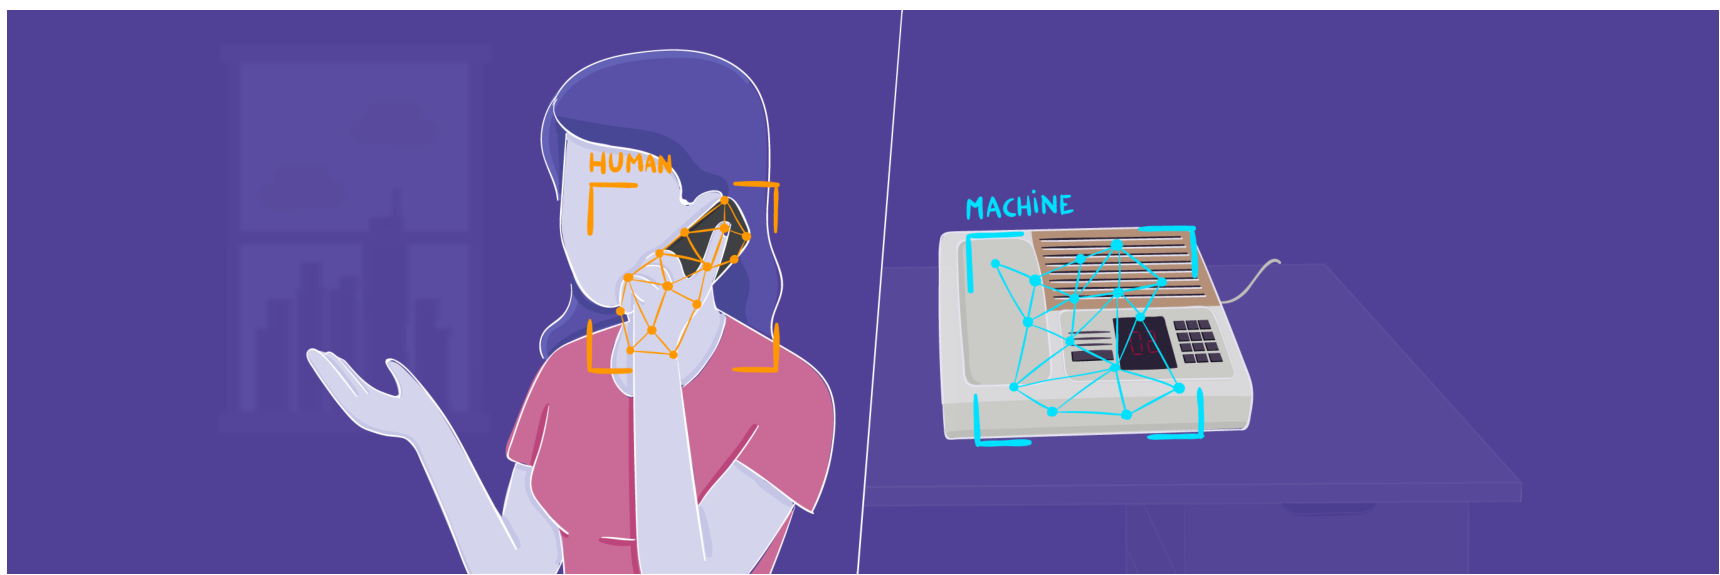
\includegraphics[width=188.16mm,height=158.30mm]{../../images/llm/page_004_img_01.png}%
\end{textblock*}

\end{document}
